\documentclass[english, a4paper, oneside, onecolumn, openany,article]{memoir}
\usepackage{fix-cm,fixltx2e}
\usepackage{babel}  % babel: Hyphenation patterns and language specific strings
\usepackage{varioref}
\usepackage[colorlinks,linkcolor=black,urlcolor=black,citecolor=black]{hyperref}
\usepackage[colorinlistoftodos]{todonotes}
\usepackage[latin1]{inputenc}
\usepackage{graphicx}
\usepackage{listings}
\usepackage[square,numbers]{natbib}
\usepackage{url}
\usepackage{pslatex}
\usepackage{multirow}
\usepackage[T1]{fontenc}
\usepackage{eso-pic}
\usepackage{xcolor,calc}
\usepackage{pdfpages}
\newsubfloat{figure}
\usepackage{placeins} % gives me FloatBarrier
%Forhindrer floats i at flyde ind i næste afsnit
\let\oldsection=\section % gemmer den gamle definition
\renewcommand\section{\FloatBarrier\oldsection}

\makeatletter
\renewcommand\fps@figure{htbp} % Force figure placement
\renewcommand\fps@table{htbp}
\makeatother

% setup captions
\hangcaption
\changecaptionwidth
\captionwidth{9cm}


\title{Advanced Data Management - Assignment 3\\Query tuning}
\author{S\o ren Bjerregaard Vrist - 151082-sbvr@itu.dk\\ \\Undervisere: Philippe
Bonnet - phbo@itu.dk og
Rasmus Pagh - pagh@itu.dk\\ITU Copenhagen}
\begin{document}
\maketitle
\newpage

\chapter{Part 1 - Query tuning}

\section{Part1a}
Baseline of the query: The query given uses an inequality ``self-join''
effectively giving a cardinality of $count\_of\_rows^2$. I use a 3.000.000 row
inkarnation of the employeespec given in assignment 2 in a table called employee2.\\
\noindent The queryplan as reported by db2expln is:
\begin{verbatim}
Estimated Cost = 77204.445312
Estimated Cardinality = 3000000.000000

Access Table Name = DB2INST1.EMPLOYEE2  ID = 2,261
|  #Columns = 6
|  Skip Inserted Rows
|  Avoid Locking Committed Data
|  Currently Committed for Cursor Stability
|  May participate in Scan Sharing structures
|  Scan may start anywhere and wrap, for completion
|  Scan can be throttled in scan sharing management
|  Relation Scan
|  |  Prefetch: Eligible
|  Lock Intents
|  |  Table: Intent Share
|  |  Row  : Next Key Share
Nested Loop Join
|  Access Table Name = DB2INST1.EMPLOYEE2  ID = 2,261
|  |  #Columns = 0
|  |  Single Record
|  |  Skip Inserted Rows
|  |  Avoid Locking Committed Data
|  |  Currently Committed for Cursor Stability
|  |  May participate in Scan Sharing structures
|  |  Scan may start anywhere and wrap, for completion
|  |  Fast scan, for purposes of scan sharing management
|  |  Scan can be throttled in scan sharing management
|  |  Relation Scan
|  |  |  Prefetch: Eligible
|  |  Lock Intents
|  |  |  Table: Intent Share
|  |  |  Row  : Next Key Share
|  |  Sargable Predicate(s)
|  |  |  #Predicates = 3
Return Data to Application
|  #Columns = 2

End of section

Optimizer Plan:

        Rows   
      Operator 
        (ID)   
        Cost   
              
       3e+06  
        n/a   
      RETURN  
       ( 1)   
      77204.4 
        |     
       3e+06  
        n/a   
      NLJOIN  
       ( 2)   
      77204.4 
     /       \-\
   3e+06        * 
    n/a        |      
  TBSCAN      3e+06   
   ( 3)        n/a    
  37813.1   Table:    
    |       DB2INST1  
   3e+06    EMPLOYEE2 
    n/a    
 Table:    
 DB2INST1  
 EMPLOYEE2 
\end{verbatim}
This shows a very big ``cost''. This
in effect means that this query will take a very long time if executed as is.

My system is an Ubuntu 9.10 on an Amazon EC2 small
\section{Part1b}
In effect the query plan says that for each row in the table we need to scan all
rows in the table at least once. If this query should be feasible the amount of
rows potential for a query should be reduced from the complete table if
possible. The last part of the query is based on latitude and longitude columns
and is in effect the euclidian distance between two points that should be less
than 10000.

\section{Part1c}
As the ``and'' part of the query is about distance in at least 2-dimensions a
specialized index might prove to help lower cardinality efficently, for example
grid files, r-trees or space filling curves. IBM provides a special extension
for DB2 for spatial indexes called ``Spatial Extender''. As described in the
logbook(Section \ref{log}) I wasnt able to install this extension. Another way
to lower cardinality might be to use the spatial distance as the first join
point before using the inequality joins on hundreds1 and hundreds2. 
For example shift the latitude and longitude down by a number thereby reducing
the precision and allowing for coarse filtering  with a ``BETWEEN'' clause:
\begin{verbatim}
SELECT
    g1.ssnum, g2.ssnum
FROM
    grid g1, grid g2
WHERE
    g2.x BETWEEN g1.x-2 AND g1.x+2 AND g2.y BETWEEN g1.y-2 AND 1.y+2 
\end{verbatim}

\section{Part1d}

This filtering gives this explain plan:
\begin{verbatim}
Statement:
  
  SELECT g1.ssnum, g2.ssnum 
  FROM m1 g1, m1 g2 
  WHERE g2.x BETWEEN g1.x-2 AND g1.x+2 AND g2.y BETWEEN g1.y-2 AND 
          g1.y+2


Section Code Page = 1208

Estimated Cost = 53848872.000000
Estimated Cardinality = 509469440.000000

Access Materialized Query Table Name = DB2INST1.M1  ID = 2,262
|  #Columns = 3
|  May participate in Scan Sharing structures
|  Scan may start anywhere and wrap, for completion
|  Scan can be throttled in scan sharing management
|  Relation Scan
|  |  Prefetch: Eligible
|  Lock Intents
|  |  Table: Intent Share
|  |  Row  : Next Key Share
Nested Loop Join
|  Access Materialized Query Table Name = DB2INST1.M1  ID = 2,262
|  |  Index Scan:  Name = DB2INST1.GIDX  ID = 1
|  |  |  Regular Index (Clustered)
|  |  |  Index Columns:
|  |  |  |  1: X (Ascending)
|  |  |  |  2: Y (Ascending)
|  |  |  |  3: SSNUM (Ascending)
|  |  #Columns = 1
|  |  Evaluate Predicates Before Locking for Committed Key
|  |  #Key Columns = 2
|  |  |  Start Key: Inclusive Value
|  |  |  |  |  1: ?
|  |  |  |  |  2: ?
|  |  |  Stop Key: Inclusive Value
|  |  |  |  |  1: ?
|  |  |  |  |  2: ?
|  |  Index-Only Access
|  |  Index Prefetch: Eligible 156
|  |  Lock Intents
|  |  |  Table: Intent Share
|  |  |  Row  : Next Key Share
|  |  Sargable Index Predicate(s)
|  |  |  #Predicates = 2
|  |  |  Return Data to Application
|  |  |  |  #Columns = 2
Return Data Completion

End of section


Optimizer Plan:

           Rows   
         Operator 
           (ID)   
           Cost   
                   
       5.09469e+08 
           n/a     
         RETURN    
          ( 1)     
       5.38489e+07 
           |       
       5.09469e+08 
           n/a     
         NLJOIN    
          ( 2)     
       5.38489e+07 
      /           \
     3e+06          * 
      n/a          |     
    TBSCAN       3e+06   
     ( 3)       Index:   
    19301.9     DB2INST1 
      |         GIDX     
     3e+06     
      n/a      
 Materialized: 
 DB2INST1      
 M1            
\end{verbatim}

This gives a reasonable view of the cost involved in the join, but is much worse than the estimated cost of the original query.

When adding this query into the orignal query(as materialized view m1) we get:
\begin{verbatim}
SELECT  distinct e1.ssnum,e1.name
FROM employees e1, employees e2,
( SELECT g1.ssnum as ssnum1, g2.ssnum as ssnum2 
  FROM  m1 g1, m1 g2 
  WHERE g2.x BETWEEN g1.x-1 AND g1.x+1 AND g2.y 
  BETWEEN g1.y-1 AND g1.y+1) as n
WHERE
  e1.ssnum = n.ssnum1  AND  e2.ssnum = n.ssnum2 AND
  (e1.hundreds1 > e2.hundreds1 or e1.hundreds2 < e2.hundreds2 )
AND
  (sqrt(bigint(e2.lat - e1.lat)*bigint(e2.lat - e1.lat) + 
   bigint(e2.long - e1.long)*bigint(e2.long - e1.long)) < 10000)
\end{verbatim}

The estimated cost of this query is massive:
\begin{verbatim}
Estimated Cost = 100864016.000000
Estimated Cardinality = 3000000.000000
\end{verbatim}
not helping at all.\\

At this point im not able to provide any further improvements.


\chapter{Part 2 - Compresssion}
\section{Part2a}
Compression is a known concept from many computer science areas and in general
the tradeoff is between disk space-usage vs. cpu. The DB2 argues that by
lowering the amount of data being compared and copies to and from memory this
tradeoff might be nulled or CPU/RAM usage be lowered as well.

\section{Part2b}
Several experiments come to mind, and the mechanial thorough student would rerun
all experiments from Assignment1 and Assignment2 to verify if compression would
slow down any of the throughput seen previously. Due to the limited time at hand
I define two experiments:
\begin{enumerate}
  \item Diskspace usage with/without compression
  \item A simple read and a simple write experiment with/without compression
\end{enumerate}
1) should show if our table structures might benefit from compression and 2)
should show if any saved disk-space hampers (or even betters our) throughput.
Take note that as I read the DB2 article on row compression the main benefits
would be from giant text databases on busy systems, neither of which is the case
with the syntetic table specs(employeespec and accountspec) and experiement
setup at hand. 

\subsection{Diskspace usage}
Before an experiment is conducted DB2 provides a tool to give an estimate as
well (db2 INSPECT ROWCOMPESTIMATE TABLE NAME employees results keep
<filename>)\\

\textbf{employee:}\\
\begin{verbatim}
Percentage of pages saved from compression: 33
Percentage of bytes saved from compression: 33
Compression dictionary size: 36736 bytes.
Expansion dictionary size: 32768 bytes.
\end{verbatim}

\textbf{accounts:}\\
\begin{verbatim}
Percentage of pages saved from compression: 24
Percentage of bytes saved from compression: 24
Compression dictionary size: 52352 bytes.
Expansion dictionary size: 32768 bytes.
\end{verbatim}

All in all, it should be possible to gain some space.

We can lookup the current usage of the tables with a lookup:
\begin{verbatim}
SELECT tabname,DATA_OBJECT_P_SIZE,INDEX_OBJECT_P_SIZE 
FROM SYSIBMADM.ADMINTABINFO where tabname in ('ACCOUNTS','EMPLOYEES')

TNAME     DATA_OBJECT_P_SIZE   INDEX_OBJECT_P_SIZE 
--------- -------------------- --------------------
EMPLOYEES               121216                20352
ACCOUNTS                 13184                 8576
\end{verbatim}

This reports that Employees is 121Mb with 20Mb indexes and accounts is 13Mb with 8Mb indexes.

After enabling compression and reorging tables:
\begin{verbatim}
TNAME     DATA_OBJECT_P_SIZE   INDEX_OBJECT_P_SIZE 
--------- -------------------- --------------------
EMPLOYEES                76416                20352
ACCOUNTS                  9984                 8576
\end{verbatim}
All in all decent disk space savings (but with small tables as this, it makes no
sense unless other benefits are occured)
\begin{verbatim}
EMPLOYEES     ~37% less space
ACCOUNTS      ~24% less space 
\end{verbatim}

\subsection{Performance}
I reuse the Parta's of assignment two and compare against the results to see if
the throughput has been affected (Scripts in Appendix \ref{app:run1rr} and
\ref{app:clustrr}.

\subsubsection{Writes}
I reran the thread experiment from assignment2(Figure 2 in assignment 2) one for a table with compression
and one without compression, trying to insert 1000000 rows with
``profwrites2.py''. Figure \ref{fig:writecomp} contains the summary of that rerun and
shows that additional overhead is
procurred when using a compressed table. In my case just about 10\%.
\begin{figure}
  \centering
  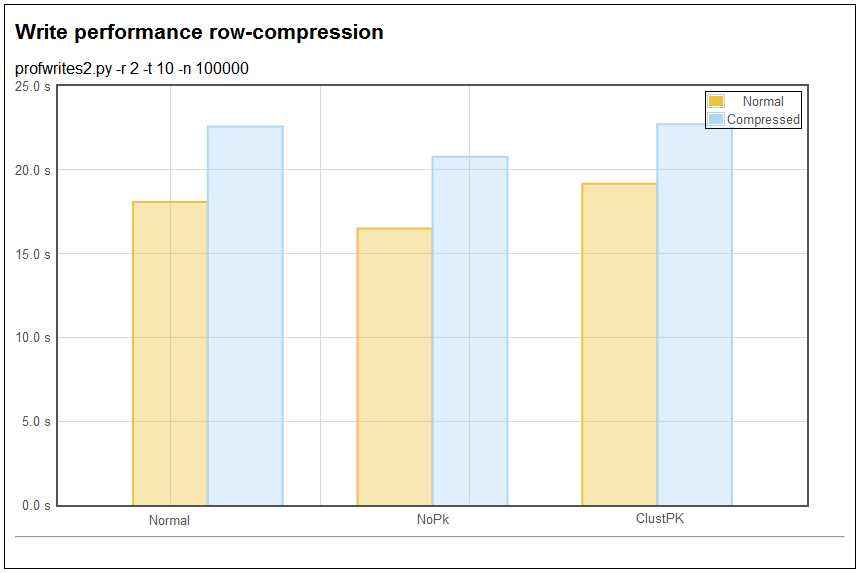
\includegraphics[width=12cm]{assignment3/writecomp}
  \caption[Write performance - compress]{Graph of write timing
  for 10 threads for either a normal table or a table with
  compression. Different index types}\label{fig:writecomp}
\end{figure}

\subsubsection{Reads}
For this experiment I reran the ``clustering index'' experiement(Figure 8 in
assignment 2) for both tables with and without compression and summarized the
results in Figure \ref{fig:readcomp}.

\begin{figure}
  \centering
  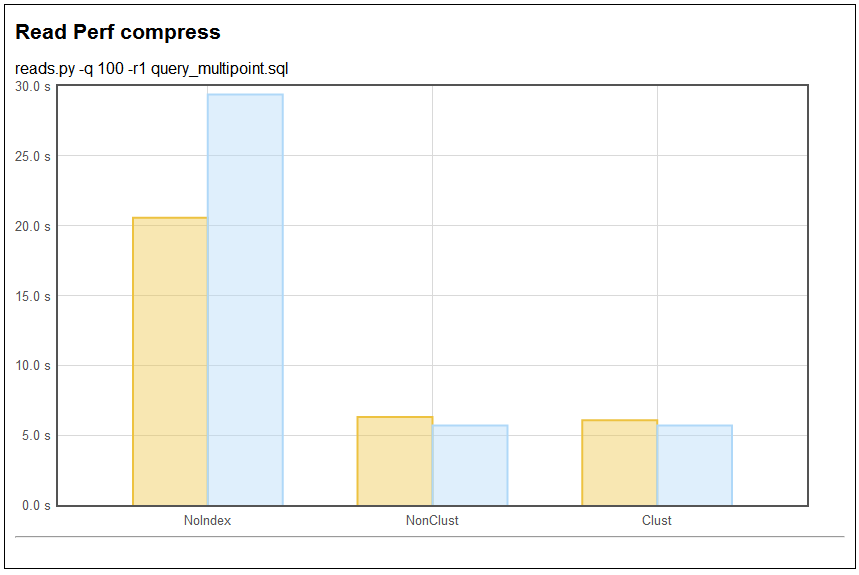
\includegraphics[width=12cm]{assignment3/readcomp}
  \caption[Read performance - Clustering Index compress]{Graph of read timing
  for 100 multipoint queries for either a normal table or a table with
  compression.}\label{fig:readcomp}
\end{figure}

Interestingly multipoint queries without indexes gets slower on a table with
compression, where tables with compression AND indexes gives faster lookup!

When comparing snapshot statistics for the queries it looks like that
compression allows for 30-40\% fewer buffer pool logical and physical reads  but
the physical reads is slower when using compression than when not. For the
indexed multipoint queries the index reduce the number of physical reads for
both data and index buffer pool and the reduction in index buffer pool physical
reads is big enough to counter the additional overhead when using compression:

\noindent\begin{tabular}{p{6.6cm}|p{6.6cm}}
  \multicolumn{2}{c}{No index}\\
No compression:&With Compression:\\ \hline
\noindent\footnotesize\protect\begin{verbatim}
Buffer pool data logical reads       = 416516
Buffer pool data physical reads      = 356819
Total buffer pool read time          = 35447
Total elapsed asynchronous read time = 34828
Asynchronous data read requests      = 11436
\end{verbatim}
&
\noindent\footnotesize\protect\begin{verbatim}
Buffer pool data logical reads       = 296927
Buffer pool data physical reads      = 262578
Total buffer pool read time          = 47058
Total elapsed asynchronous read time = 44836
Asynchronous data read requests      = 8570
\end{verbatim}
\\ \hline
\end{tabular}


\noindent\begin{tabular}{p{6.6cm}|p{6.6cm}}
  \multicolumn{2}{c}{NonClustering Index}\\
  No compression:&With Compression:\\ \hline
\noindent\footnotesize\begin{verbatim}
Buffer pool data logical reads       = 230436
Buffer pool data physical reads      = 7455
Asynchronous pool data page reads    = 7262
Buffer pool index logical reads      = 10406
Buffer pool index physical reads     = 4486
Total buffer pool read time          = 8242
Total elapsed asynchronous read time = 2282
\end{verbatim}
&
\noindent\footnotesize\begin{verbatim}
Buffer pool data logical reads       = 198195
Buffer pool data physical reads      = 4799
Asynchronous pool data page reads    = 4720
Buffer pool index logical reads      = 3513
Buffer pool index physical reads     = 1143
Total buffer pool read time          = 4543
Total elapsed asynchronous read time = 1459
\end{verbatim}
\\ \hline
\end{tabular}




\chapter{Log book over experiments}\label{log}
\section{Part 1}
\begin{itemize}
\item[2010-04-08:] Spent all day trying to install spatial extensions for db2.
To no avail. The installer cant see which BASE\_DB2\_ENGINE is installed. The
\verb|db2ls -q -b <something>| is empty
\item[2010-04-09:] Got hint from Thomas Berglund in the newsgroup about how to
  lower cardinality.
\end{itemize}

\section{Part2}
\begin{itemize}
\item[2010-04-09:] Having trouble estimating disk usage of a database as DB2
  reserves space on disk even though it might not be used at present. Using the
  indicators from within DB2 instead of du(1)
\end{itemize}
\appendix
\newpage
\chapter{Appendix}

\section{run1-Rerun.bash - Write script}\label{app:run1rr}
\lstinputlisting{assignment3/run1-rerun.bash}

\section{clustrerun.bash - Write script}\label{app:clustrr}
\lstinputlisting{assignment3/clustrerun.bash}

\end{document}
